\section{Android系统架构}
Android是由Google开发的一种移动操作系统, 该系统基于修改后的Linux内核构建, 由5层结构的软件栈构成, 如图\ref{androidStructure}所示\juhao
\begin{figure}[ht]
	\centering
	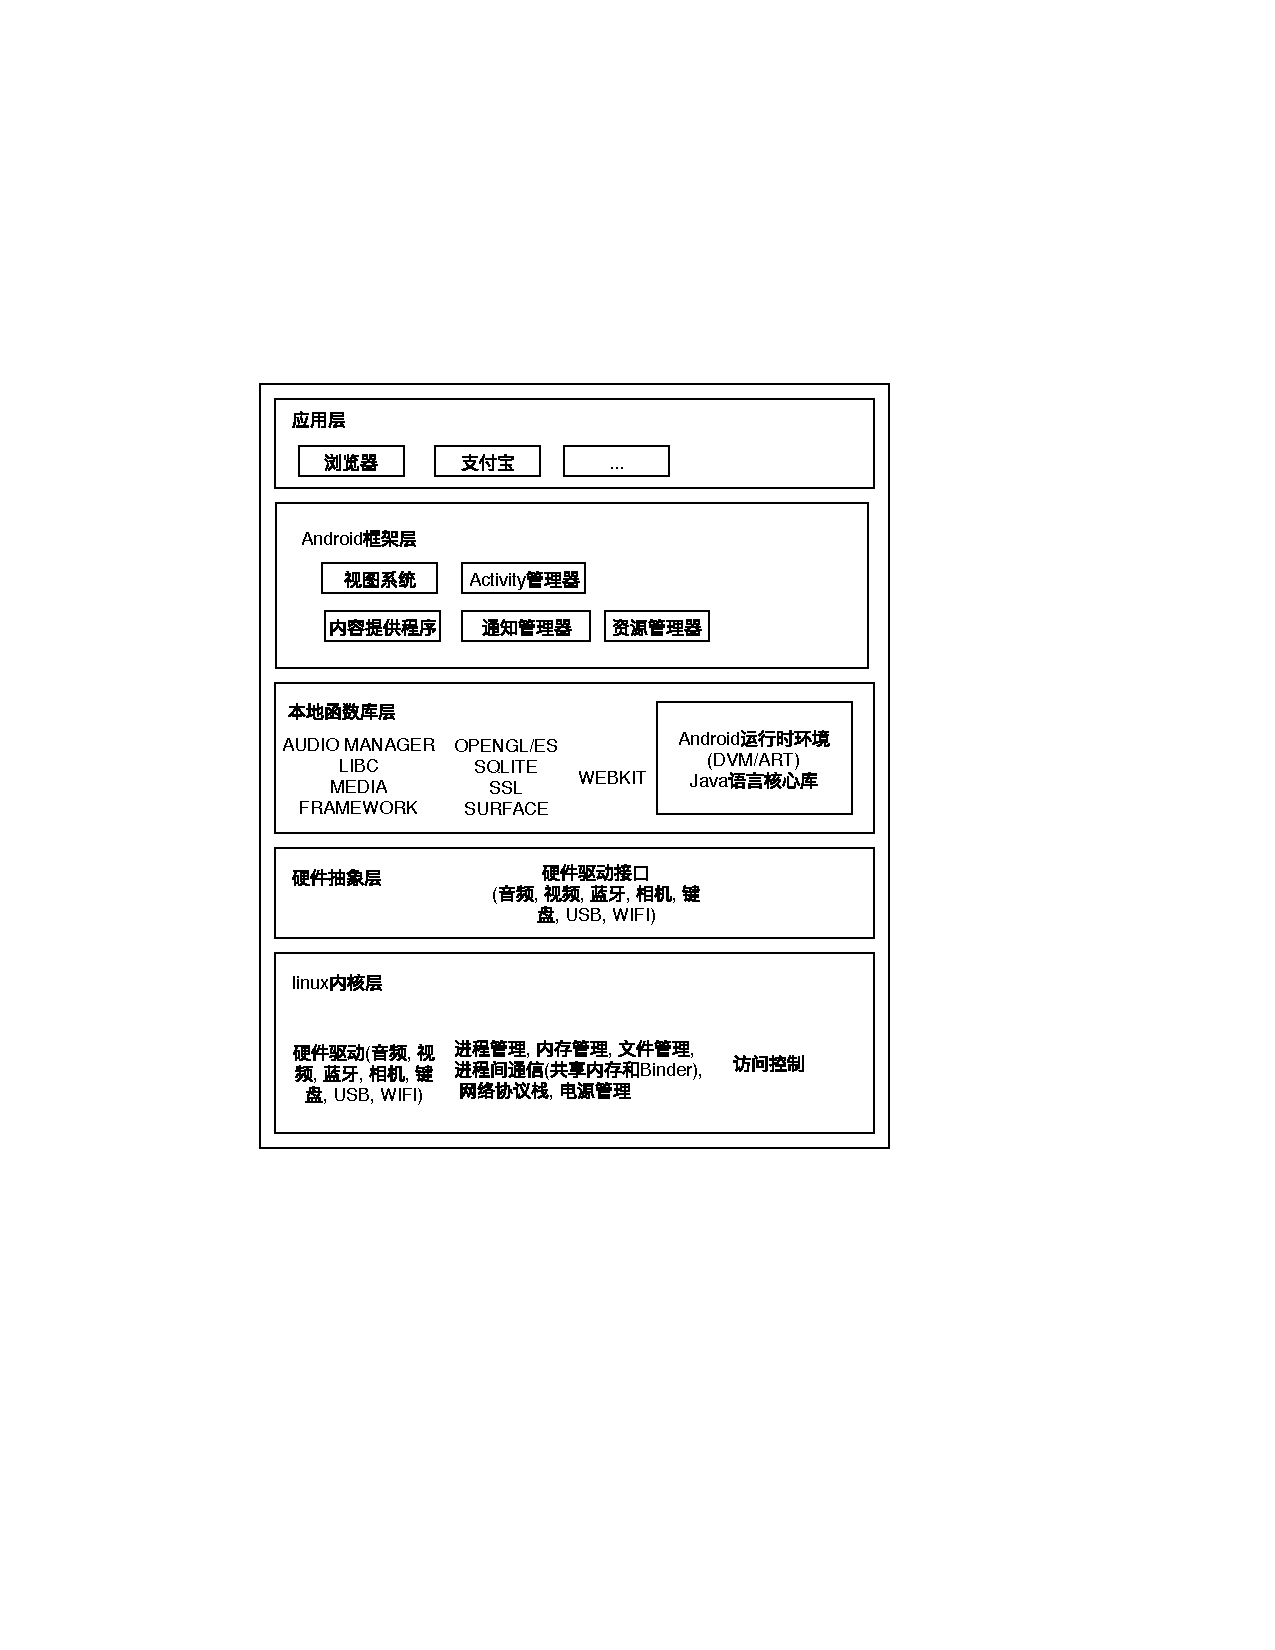
\includegraphics[width=\textwidth]{android_structure.jpg}
	\caption{Android系统架构}
	\label{androidStructure}
\end{figure}

\section{Android应用结构}
\section{Android动态分析技术}
\section{Android加壳和混淆技术}
\section{Android Runtime}
\subsection{简介}
\subsection{应用的启动}
\subsection{应用的加载}
\subsection{方法的执行}
\section{frida框架}
